\documentclass[a4paper,11pt]{article}
\usepackage[T1]{fontenc}
\usepackage[utf8]{inputenc}
\usepackage{lmodern}
\usepackage[francais]{babel}

% title info
\newcommand{\ititle}{Cahier des Charges NF28} % title
\newcommand{\isubtitle}{Projet Colladia \\(Collaborative Diagrams)}
\newcommand{\iauthor}{IMPELLETTIERI Florian
						\\VINTACHE Jean
						\\HAMMI Marouane
						\\MENIER Charles
						} % author
\newcommand{\idate}{\today} % date

\usepackage{graphicx}
\usepackage{tabularx}
\usepackage{lastpage}
\usepackage[top=2.75cm, bottom=3cm, left=2cm, right=2cm]{geometry}
\usepackage[colorlinks=true, urlcolor=blue, linkcolor=black, citecolor=black]{hyperref}
\usepackage{calc}
\usepackage{amsmath} % equation align
\usepackage{amsfonts}
\usepackage{amssymb}
\usepackage{fancyhdr}
\usepackage[format=hang, width=.8\textwidth, labelfont=sc]{caption}
\usepackage[format=hang, width=.8\textwidth, labelfont=normalfont]{subcaption}
% \usepackage[labelformat=empty]{caption} % no label before caption
\usepackage{verbatim}

% paragraph and subparagraph as level 4 and 5 sections
\usepackage{titlesec}
\usepackage{titletoc}
\setcounter{secnumdepth}{5}
\setcounter{tocdepth}{5}
\titleformat{\paragraph} [hang] {\normalfont\normalsize\bfseries} {\theparagraph} {1em} {}
\titleformat{\subparagraph} [hang] {\normalfont\normalsize\bfseries} {\thesubparagraph} {1em} {}

% lists config
\usepackage{enumitem}
\setlist[itemize]{label=-}

% replace no-break space
\DeclareUnicodeCharacter{00A0}{ }

% header & footer
\pagestyle{fancy}
\fancyhf{}
\setlength{\headheight}{14pt}
\lhead{{\small \ititle}}
\rhead{{\small \isubtitle}}
\lfoot{}
\rfoot{\hrule\vspace{.1cm}\thepage /\pageref*{LastPage}}

\usepackage{color}
\usepackage{xcolor}
\usepackage{listings}

% define colors
\definecolor{kblue}{HTML}{204A87}
\definecolor{cred}{HTML}{A52A2A}
\definecolor{sorange}{HTML}{FF7800}
\definecolor{ngreen}{HTML}{4E9A06}
\definecolor{pprocess}{HTML}{339999}
\definecolor{opbrown}{HTML}{AB7A00}

% code highlight style
\lstdefinestyle{lstyle}{
	aboveskip=9mm,
	belowskip=1mm,
	basicstyle=\ttfamily\footnotesize,
	keywordstyle=\bfseries\color{kblue},
	commentstyle=\color{cred},
	stringstyle=\color{sorange},
	emphstyle=\color{pprocess},
	breaklines=true,
	tabsize=3,
	showstringspaces=false,
	captionpos=b
% 	literate={=}{{{\color{opbrown}=}}}1
}

% language
\lstset{
	language=Java,
	frame=single,
	numbers=left,
	numberstyle=\footnotesize,
	style=lstyle,
	emph={},
	morekeywords={None, False, True},
	extendedchars=true
}

% utf8 char
\lstset{literate=
  {á}{{\'a}}1 {é}{{\'e}}1 {í}{{\'i}}1 {ó}{{\'o}}1 {ú}{{\'u}}1
  {Á}{{\'A}}1 {É}{{\'E}}1 {Í}{{\'I}}1 {Ó}{{\'O}}1 {Ú}{{\'U}}1
  {à}{{\`a}}1 {è}{{\`e}}1 {ì}{{\`i}}1 {ò}{{\`o}}1 {ù}{{\`u}}1
  {À}{{\`A}}1 {È}{{\'E}}1 {Ì}{{\`I}}1 {Ò}{{\`O}}1 {Ù}{{\`U}}1
  {ä}{{\"a}}1 {ë}{{\"e}}1 {ï}{{\"i}}1 {ö}{{\"o}}1 {ü}{{\"u}}1
  {Ä}{{\"A}}1 {Ë}{{\"E}}1 {Ï}{{\"I}}1 {Ö}{{\"O}}1 {Ü}{{\"U}}1
  {â}{{\^a}}1 {ê}{{\^e}}1 {î}{{\^i}}1 {ô}{{\^o}}1 {û}{{\^u}}1
  {Â}{{\^A}}1 {Ê}{{\^E}}1 {Î}{{\^I}}1 {Ô}{{\^O}}1 {Û}{{\^U}}1
  {œ}{{\oe}}1 {Œ}{{\OE}}1 {æ}{{\ae}}1 {Æ}{{\AE}}1 {ß}{{\ss}}1
  {ç}{{\c c}}1 {Ç}{{\c C}}1 {ø}{{\o}}1 {å}{{\r a}}1 {Å}{{\r A}}1
  {€}{{\EUR}}1 {£}{{\pounds}}1
}

% use with \begin{lstlisting}[caption={#}, language=#] # \end{lstlisting}
% or \lstinline[caption={#}, language=#]$#$ --> $ can be replaced by any other character not used in the code


\begin{document}
% title
\newcommand*{\ClipSep}{0.4cm}
\begin{center}
	\hspace*{-1.8cm}
	\begin{tikzpicture}
		\node [inner sep=0pt] at (0,0) {
\includegraphics[width=\textwidth+3cm]{img/colladia-banner}};
		\draw [white, rounded corners=\ClipSep, line width=\ClipSep] 
				(current bounding box.north west) -- 
				(current bounding box.north east) --
				(current bounding box.south east) --
				(current bounding box.south west) -- cycle
				;
	\end{tikzpicture}~\\\vspace*{.5cm}
% 	\vspace*{.75cm}{\huge \textsc{\ititle}}~\\
% 	\vspace{.25cm}{\LARGE \isubtitle}~\\
	\vspace{1cm}{\large\iauthor}~\\
	\vspace{.6cm}{\large\idate}
\end{center}
\vspace*{-1.5cm}

% table of content (titlepage)
% \vspace{\fill}
% \tableofcontents

% logo
\vspace{\fill}
\hspace{-1.25cm}
\includegraphics[width=5cm]{img/utc-logo.jpg}
\vspace*{-1.5cm}

\thispagestyle{empty}

% table of content (newpage)
\newpage
\tableofcontents

% blue links after table of contents
\hypersetup{linkcolor=blue}

% section config
\titlespacing{\section}{0mm}{6mm}{0mm}
\titlespacing{\subsection}{0mm}{6mm}{0mm}
\titlespacing{\subsubsection}{0mm}{6mm}{0mm}
\titlespacing{\paragraph}{0mm}{6mm}{0mm}
\titlespacing{\subparagraph}{0mm}{6mm}{0mm}

% paragraph config
\setlength{\parindent}{0mm}
\setlength{\parskip}{6mm}


\newpage
\section{Introduction}
Ce document constitue le cahier des charges du projet de NF28. Au cours de ce projet l'objectif sera de proposer à des utilisateurs une expérience d'interaction agréable. Ceci à travers une interface graphique ergonomique adapté aux besoins utilisateurs.

\subsection{Équipe}
Notre groupe est composé de 5 étudiants :
\begin{itemize}
\item IMPELLETTIERI Florian (NF28/IA04)
\item VINTACHE Jean (NF28/IA04)
\item JACQUET Adrien (IA04)
\item HAMMI Marouane (NF28/IA04)
\item MENIER Charles (NF28)
\end{itemize}
\section{Description}
Le but du projet sera de créer un logiciel de tableau blanc collaboratif, qui permettrait de générer diverses formes, pour réaliser des diagrammes ou des schémas.
Le projet sera couplé avec celui d'IA04, ce qui nécessitera de mettre en place des agents. Il se destine aux appareils mobiles (smartphones et tablettes). Une attention sera donc portée à la facilité d’utilisation sur des écrans relativement petits et tactiles.
\section{Intérêt principal}
On dit qu’un dessin vaut mieux qu’un long discours. Partant de ce principe, l’objectif de Colladia serait de proposer aux utilisateurs une expérience leur permettant de pouvoir dessiner ensemble chacun sur leur propre appareil mobile. 

Les utilisateurs peuvent ainsi modifier le document simultanément, et profiter des interactions tactiles qu’offre ces supports.

\section{Utilisateurs visés}

Les premiers utilisateurs visées seront notamment les étudiants et des professionnels qui rencontrent la nécessité de réaliser des diagrammes UML dans leur quotidien.
L'application sera axé sur ces utilisateurs pour proposer des éléments de diagramme adaptés à leur besoins.

\section{Étude des utilisateurs (interviews, enquêtes)}
TODO

\newpage
\section{Étude de quelques logiciels concurrents}
Lors de nos recherches, deux application semblaient réellement en concurrence avec notre solution. À savoir draw.io de Google et DrawExpress de DrawExpress Inc.

\subsection{Draw.io}
Néanmoins draw.io, bien que collaboratif n'utilise pas pleinement les fonctionnalités tactiles des supports mobiles.

\begin{figure}[h]
	\centering
	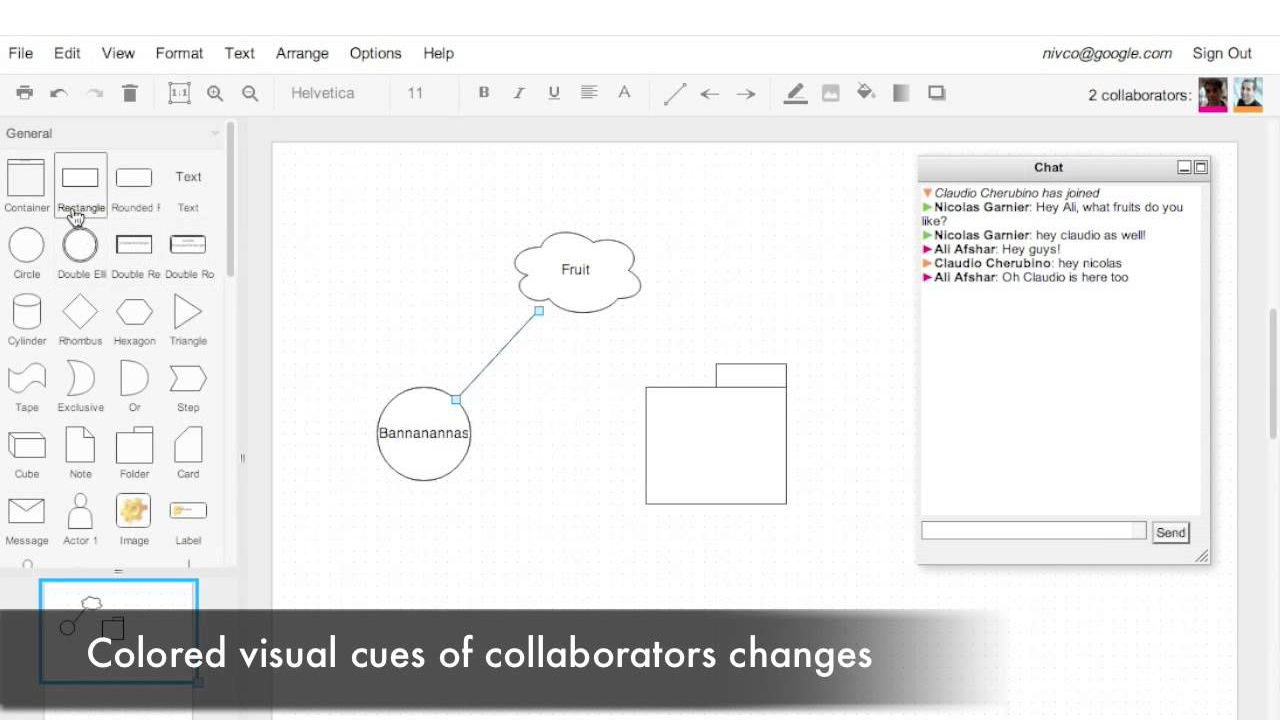
\includegraphics[width=15cm]{img/drawio.PNG}
	\caption{draw.io - Édition en collaboration}
\end{figure}


\subsection{DrawExpress}
Ce que fait DrawExpress c’est de proposer une éditeur de diagramme sur mobile. Il est cross-plateforme (IOS, Android et BlackBerry) mais il ne permet pas la travail simultané à plusieurs.

\begin{figure}
	\centering
	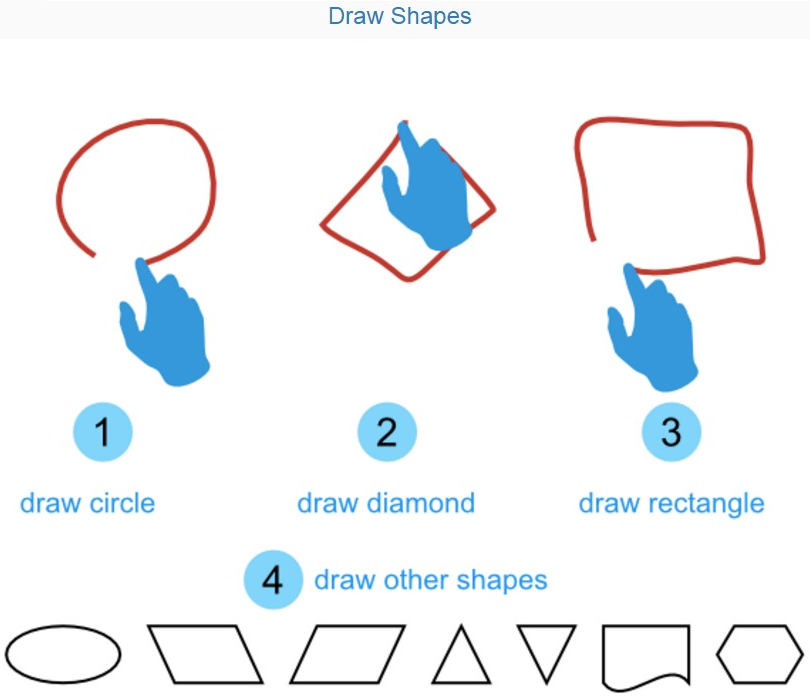
\includegraphics[width=10cm]{img/DrawExpressRecognition.PNG}
	\caption{Aperçu des interactions tactiles de DrawExpress - \\Reconnaissance de forme}
\end{figure}

\begin{figure}
	\centering
	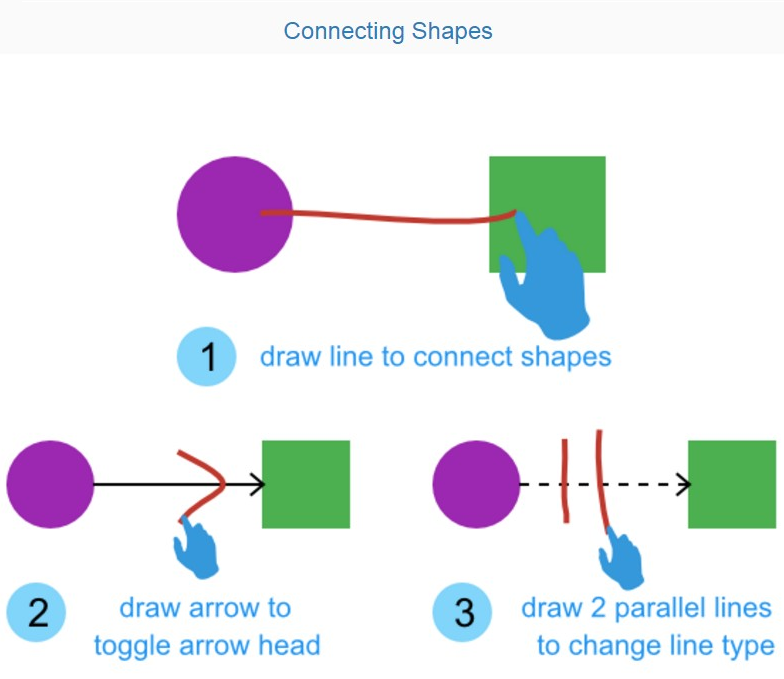
\includegraphics[width=10cm]{img/DrawExpressLinks.PNG}
	\caption{Aperçu des interactions tactiles de DrawExpress - Tracé de lignes}
\end{figure}

Cette application constitue une bonne base d’inspiration pour Colladia puisqu’elle est utilise particulièrement les interactions tactiles permises par les smartphones afin de créer, à partir de gestes simples à main levée, des formes prédéfinies qui constituent le diagramme construit. De cette manière, l’ergonomie est optimisée pour les écrans tactiles et de petite taille.

\subsection{Positionnement}

Le but de Colladia est donc de proposer les deux points forts ces deux logiciels concurrents, à savoir le travail collaboratif et les interactions tactiles.


\section{Fonctionnalités}
\subsection{Fonctionnalités générales}
	\begin{itemize}
		\item Connexion au serveur avec pseudo
		\item Création d'un nouveau diagramme
		\item Rejoindre un diagramme parmi une liste de diagrammes existants
		\item Déplacement de la vue sur le diagramme
		\item Ajout, Suppression et Modification d'éléments
	\end{itemize}
\subsection{Fonctionnalités tactiles}

\begin{itemize}
\item Icône transparent dans le coin pour ouvrir le menu
\item Ajout de formes prédéfinies (Classes UML, cercles, carrés, rectangles,...)
\item Liste des utilisateurs présent sur un même diagramme :
\begin{itemize}
	\item Possibilité de suivre un utilisateur
	\item Affichage de la vue d’un utilisateur
\end{itemize}

\item Un appui long sur un élément permet d’ouvrir un menu contextuel spécifique à l’élément :
\begin{itemize}
	\item Mettre au premier ou au dernier plan l’élément
	\item Attirer l’attention des autres utilisateurs (à l’aide d’une flèche)
	\item Permettre : la modification ou la suppression de l’élément
\end{itemize}

\item Un appui long dans le vide permet d’ajouter des éléments
\item Un “double-tap” à 2 doigts permet de  passer du mode dessin au déplacement (et inversement)
\item Un mouvement de slide permet de se déplacer sur la zone de dessin

\begin{itemize}
	\item si un élément est sélectionné alors on déplace ce dernier
\end{itemize}

\item Un appui sur un élément le sélectionne
\begin{itemize}
	\item en appuyant de nouveau sur un élément sélectionné ou sur un espace vide, on dé-sélectionne l'élément
\end{itemize}

\item Le mouvement de pinch habituel pour gérer les effets de zoom
\begin{itemize}
	\item si élément est sélectionné, ce mouvement peut aussi servir de redimensionnement 
\end{itemize}

\end{itemize}


\subsection{Fonctionnalités optionnelles}
Compte tenu des contraintes de temps imposé par le projet, il ne nous est pas possible d'entreprendre les différentes idées que nous avons eu pour améliorer l'expérience utilisateur.

Néanmoins, voici certaines améliorations que nous essayerions d'apporter à l'application dans la mesure du possible.

\begin{itemize}
\item un chat pour laisser la possibilité aux membres de communiquer
\item l’utilisation de commandes vocales pour faciliter l’utilisation de l’application
\item un système de commentaire sur les diagrammes, pour fournir des informations complémentaires
\item une fonction de recherche de texte
\item la fusion de diagramme
\item l’exportation des diagrammes sous différents formats
\item la gestion des utilisateurs et des droits
\item la gestion des sauvegardes (automatique côté serveur)
\item le dessin à main levé qui permet une reconnaissance de forme et d’ajout d’élément automatiquement

\end{itemize}


\section{Technologies}
Afin de proposer une application collaborative, la décision de réaliser une application client serveur a rapidement été prise.

\subsection{Côté serveur}
Le projet étant couplé avec celui de IA04, il faudra mettre en place un serveur sur lequel tournera une plateforme multi-agent, à savoir JADE. 
Une API REST sera mise en place pour communiquer avec les différents clients.

\subsection{Côté client}
L’utilisateur aura accès à l’application sur une tablette ou un smartphone.  
Le développement sur ces terminaux peut être réalisé de différentes manières.
\begin{itemize}
\item en natif : il aurait alors fallu développer en code natif directement. Ce type de développement oblige un travail de développement important pour le proposer sur diffèrent systèmes d’exploitation (iOS, Android,...). Cependant l’application réalisé est plus performante.
\item en utilisant xamarin : ce mode de développement permet de générer du code natif dans les diverses plateformes existantes que ce soit iOS, Android ou WindowsPhone. 
\item en utilisant cordova : le code obtenu donne l’aspect d’une application, mais il s’agit en réalité d’une webview. L’application peut aussi se révéler moins performante qu’une application native.

\end{itemize}

Après concertation il a été décidé de réaliser l’application cliente avec Xamarin.
\begin{figure}
	\centering
	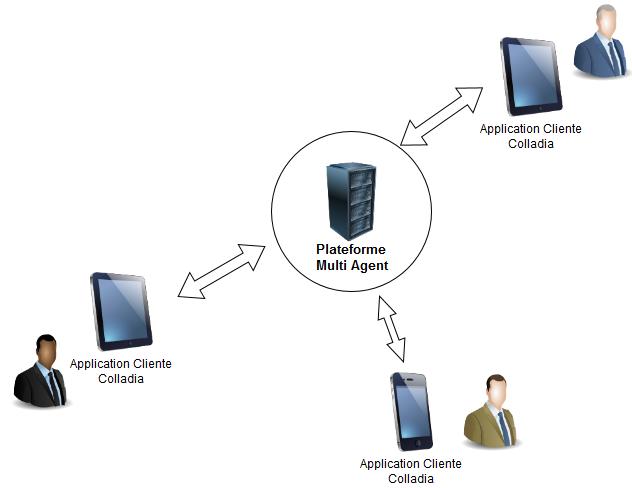
\includegraphics[width=10cm]{img/Archi.PNG}
	\caption{Schéma de l’architecture de Colladia : Client/Serveur}
\end{figure}

% Commentaires
\end{document}
